\documentclass[11pt, oneside]{article} 
\usepackage{geometry}
\geometry{letterpaper} 
\usepackage{graphicx}
	
\usepackage{amssymb}
\usepackage{amsmath}
\usepackage{parskip}
\usepackage{color}
\usepackage{hyperref}

\graphicspath{{/Users/telliott_admin/Tex/png/}}
% \begin{center} 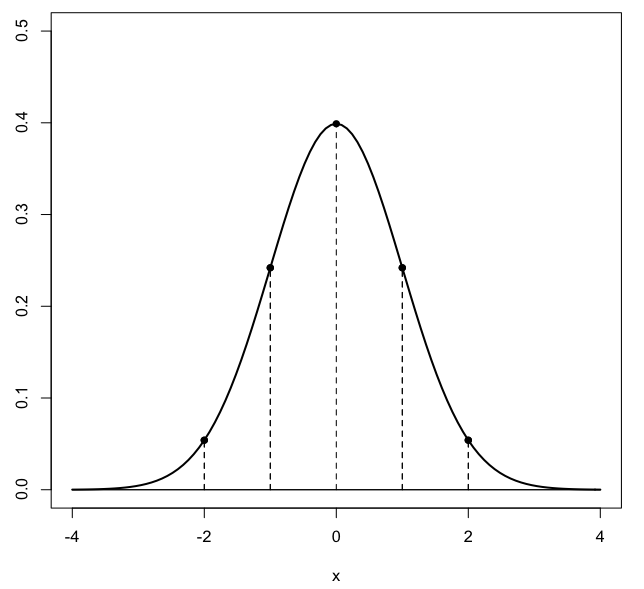
\includegraphics [scale=0.4] {gauss3.png} \end{center}

%break
\title{Implicit differentiation}
\date{}

\begin{document}
\maketitle
\Large
\label{sec:Techniques_of_differentiation}

\label{sec:Implicit_differentiation}

In this section we take a look at implicit differentiation, a remarkably powerful technique.

We will prove that the power rule $d/dx \ x^n = n x^{n-1}$ applies not only for integer $n$, both positive and negative, but also for rational $n$ like $\sqrt{x}$ or $1/x^{3/2}$.

\section*{Implicit differentiation}
Suppose we have a circle of radius $R$ with equation
\[ x^2 + y^2 = R^2 \]
\[ y = \sqrt{R^2 - x^2} \]

We'd like to find the derivative.  It is not too hard by the standard method.  By the chain rule
\[ y' = \frac{1}{2} \ \frac{1}{\sqrt{R^2 - x^2}} (-2x) = -\frac{x}{y} \]

But there is another way.  
\[ x^2 + y^2 = R^2 \]
Take $d/dx$ of all the terms on both sides.  The right-hand side is a constant so
\[ 2x + \frac{d}{dx} \ y^2 = 0 \]
By the chain rule:
\[ 2x + 2y \ \frac{dy}{dx} = 0 \]
\[ \frac{dy}{dx} = - \frac{x}{y} \]

We can also imagine a new variable, call it a parameter $t$ where 
\[ x = t \]
Think of $t$ like ticks of a clock and $x$ has been scaled to follow $t$ exactly.

Since $y$ is a function of $x$ and $x$ is a function of $t$, $y$ is also a function of $t$.
\[ y = f(t) \]

Now differentiate with respect to $t$, using the chain rule:
\[ x^2 + y^2 = R^2 \]
\[ 2x \ \frac{dx}{dt} + 2 y \ \frac{dy}{dt} = 0 \]
It is OK to multiply by $dt$
\[ x \ dx + y \ dy = 0 \]
\[ \frac{dy}{dx} = -\frac{x}{y} \]

If you find the idea of a parametric equation confusing, read ahead to \hyperref[sec:Parametric_equations]{\textbf{this chapter}}.

After a while you will not need the parameter or even the chain rule.  Just say
\[ x^2 + y^2 = R^2 \]
\[ 2x \ dx + 2y \ dy = 0 \]
and so on.

Equivalent statements:
\[ 2x + 2y \ \frac{dy}{dx} = 0 \]
\[ 2x + 2y \ y' = 0 \]

\subsection*{derivative of the cosine}

To obtain
\[ \frac{d}{dx} \ \cos x \]

we originally set up a difference quotient.  Here is another way using implicit differentiation and the chain rule.

Start from
\[ \sin^2 x + \cos^2 x = 1 \]
\[ 2 \sin x \ (\frac{d}{dx} \sin x) + 2 \cos x \ (\frac{d}{dx} \cos x) = 0 \]

Plugging in for the derivative of $\sin x$:
\[ 2 \sin x \cos x + 2 \cos x (\frac{d}{dx} \cos x) = 0 \]
\[ \sin x + (\frac{d}{dx} \cos x) = 0 \]
Rearranging, we obtain
\[ \frac{d}{dx} \cos x = - \sin x \]

\subsection*{power rule}

We can use implicit differentiation to prove that the power rule is correct for rational exponents:
\[ y = x^{m/n} \]
\[ y^n = x^m \]

Differentiate implicitly:
\[ n y^{n-1} \ dy = mx^{m-1} \ dx \]
\[ \frac{dy}{dx} = \frac{mx^{m-1} }{n y^{n-1}} \]
\[ = \frac{m}{n} \ \frac{x^{m-1}}{(x^{m/n})^{n-1}} \]
\[ = \frac{m}{n} \ \frac{x^{m-1}}{x^{m - m/n}} \]
Add up the exponents of $x$:
\[ (m - 1) - (m - \frac{m}{n} ) = \frac{m}{n} - 1\]
The result is the power rule.
\[ \frac{d}{dx} \ x^{m/n} = \frac{m}{n} \ x^{m/n - 1} \]

Later we will use logarithmic differentiation to show that it applies for \emph{any real number} $n$.  That's quite impressive.

\subsection*{example}
Consider the hyperbola
\[ xy = c \]
where $c$ is a constant.  The standard approach would be
\[ y = \frac{c}{x} \]
\[ \frac{dy}{dx} = y' = -\frac{c}{x^2} \]

Implicit differentiation:
\[ \frac{d}{dx} \ xy = \frac{d}{dx} \ c = 0 \]
\[ (xy)' = x \ y' + y \ x' = 0  \]
\[ xy' + y = 0 \]
\[ y' = -\frac{y}{x} \]
\[ = -\frac{c}{x^2} \]

\subsection*{example}
Suppose we have the equation of a tilted ellipse:
\[ x^2 - xy + y^2 = 3 \]

\begin{center} 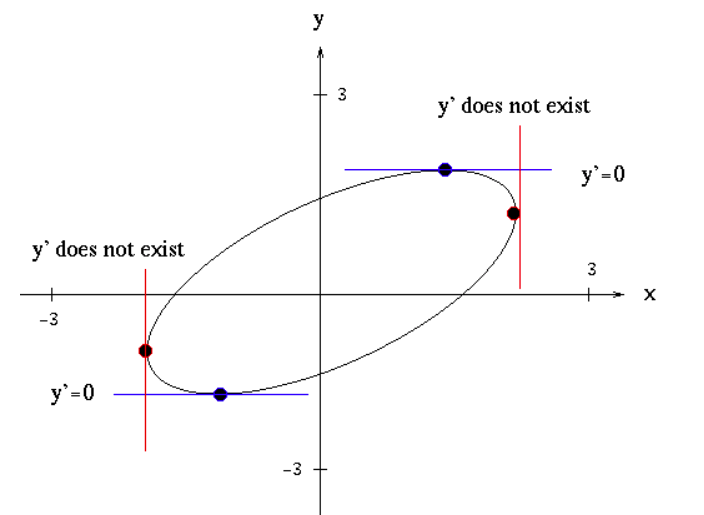
\includegraphics [scale=0.4] {tilted_ellipse2.png} \end{center}

The problem asks us to find the extreme values of $x$ and $y$ on this ellipse.  We take derivatives implicitly using the product rule on the second term:

\[ x^2 - xy + y^2 = 3 \]
\[ 2x \ dx - (x \ dy + y \ dx) + 2 y \ dy = 0 \]
\[ 2x \ dx - y \ dx = - 2y \ dy + x \ dy \]
\[ \frac{dy}{dx} = \frac{2x - y}{-2y + x} \]

Set $y'$ equal to $0$:
\[  -\frac{2x - y}{2y - x} = 0 \]

The extremes of $y$ occur when $y' = 0$, that is when
\[ y = 2x \]

Substituting $y = 2x$ into the original equation we obtain
\[ x^2 - 2x^2 + 4x^2 = 3 \]
\[ x^2 = 1 \]
\[ x = \pm \ 1 \]

Substituting again ($x = \pm \ 1$) into the original equation
\[ 1 - y + y^2 = 3 \]
\[ y^2 - y - 2 = 0 \]
\[ (y - 2)(y + 1) = 0 \]
\[ y = 2, -1 \]

On the other hand, the maximum values of $x$ occur when $y'$ does not exist:
\[ 2y = x \]
By symmetry, I claim that this occurs when $y = \pm \ 1$, with analogous solutions for $x$.

\subsection*{example}

Hamming asks us to find the angles at which two curves meet in the first quadant.

\begin{center} 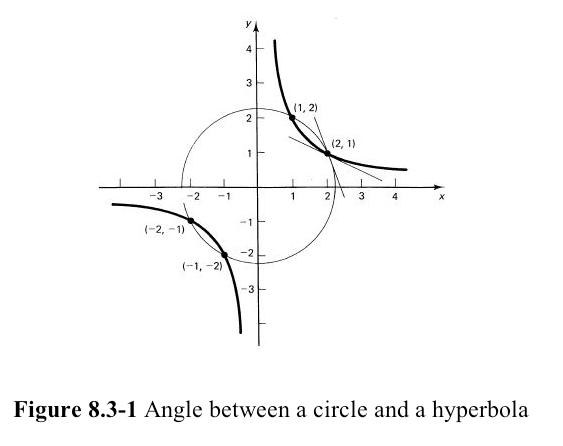
\includegraphics [scale=0.6] {two_curves.png} \end{center}

The first step is to find the points where the curves meet.

\[ x^2 + y^2 = 5 \]
\[ xy = 2 \]

so

\[ x^2 + (\frac{2}{x})^2 = 5 \]
\[ x^4 + - 5x^2 + 4 = 0 \]
\[ x^2 = \frac{5 \pm \ \sqrt{25 - 16}}{2} \]
\[ = \frac{5 \pm \ 3}{2} = 1, 4 \]
\[ x = 1, 2 \]

The corresponding points are $(1,2)$ and $(2,1)$.

We have missed two other solutions.  This happened when we took the positive square root of $x$ at the last step.  However, we are only interested in the first quadrant, so we can ignore those two for now.

Hamming solves this a bit differently, instead, he says to add and subtract $2xy = 4$ from the equation of the circle
\[ x^2 + 2xy + y^2 = 9 \]
\[ (x + y)^2 = 9 \]
\[ x + y = \pm \ 3 \]
and
 \[ x^2 - 2xy + y^2 = 1 \]
\[ (x - y)^2 = 1 \]
\[ x - y = \pm \ 1 \]

This leads to the same two answers in the first quadrant:  $(2,1)$ and $(1,2)$.

We're not done yet.  We need the angles.  

\subsection*{angle between two lines}

Consider two lines with slopes $m_1$ and $m_2$ which make angles $\theta_1$ and $\theta_2$ with the positive $x$-axis.  They meet at a point, forming the angle $\theta$, which we take to be the angle through which the first line is rotated counter-clockwise to meet the second.

\begin{center} 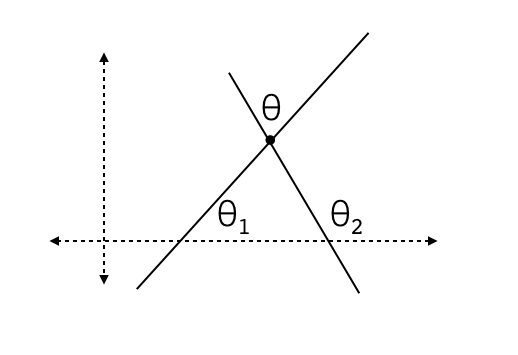
\includegraphics [scale=0.5] {two_lines2.png} \end{center}

You should be able to show that $\theta_1 + \theta = \theta_2$.

Look at the triangle formed by the two lines and the $x$-axis.  The (unlabeled) upper angle is equal to $\theta$, by the vertical angles theorem.  Therefore $\theta + \theta_1$ plus the (unlabeled) angle at the right side of the triangle add up to 180 degrees.  But $\theta_2$ plus this angle is also equal to 180 degrees, by the supplementary angles theorem.

We have then
\[ \theta_1 + \theta = \theta_2 \]
\[ \theta = \theta_2 - \theta_1 \]

The slope of a line is equal to the tangent of the angle the line makes with the $x$-axis.  

We'll see the connection in a bit, for now, we just convert the above relationship between angles with what we know in the original problem, slopes, by taking the tangent of both sides:
\[ \tan \theta = \tan(\theta_2 - \theta_1) \]

We need the sum (difference) of angles formula for the tangent.  

\subsection*{sum of angles, tangent}

From the sum of angles for sine and cosine we can write
\[ \tan s + t = \frac{\sin s + t}{\cos s + t} = \frac{\sin s \cos t + \cos s \sin t}{ \cos s \cos t - \sin s \sin t} \]
Dividing by $\cos s \cos t$ we obtain
\[ \tan s + t = \frac{\tan s + \tan t}{1 - \tan s \tan t} \]
Exchanging $-t$ for $t$ changes the sign of the tangent
\[ \tan s - t = \frac{\tan s - \tan t}{1 + \tan s \tan t} \]

We had
\[ \tan \theta = \tan(\theta_2 - \theta_1) \]
so
\[ \tan \theta = \tan(\theta_2 - \theta_1) = \frac{\tan  \theta_2 - \tan  \theta_1}{1 + \tan  \theta_1 \tan  \theta_2} \]

\subsection*{finishing up}

We said that the slope of a line is equal to the tangent of the angle the line makes with the $x$-axis.  Therefore, we can substitute slopes for tangents
\[ \tan \theta = \frac{m_2 - m_1}{1 + m_1 m_2} \]

And now we're finally ready to solve the problem we were originally given.  We use implicit differentiation to obtain the slopes of the circle and the ellipse, both of which we did earlier.  

Suppose we call the hyperbola curve $1$

\begin{center} 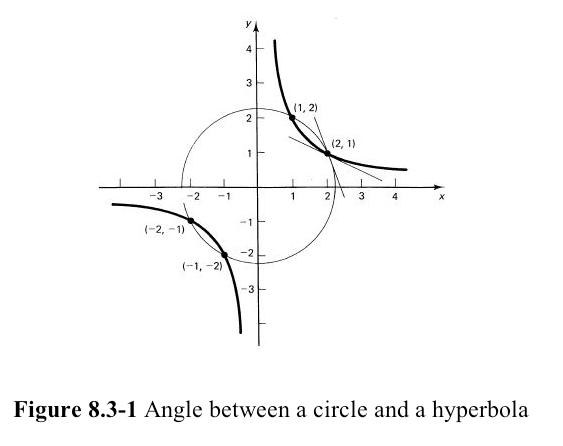
\includegraphics [scale=0.6] {two_curves.png} \end{center}

It has slope (at the point $(2,1)$):
\[ m_1 = y' = -\frac{2}{x^2} = - \frac{1}{2} \]

The circle at the point $(2,1)$ has slope:
\[ m_2 = y' =  -\frac{x}{y} = - 2 \]
This is quite reasonable, if you look at the diagram.  So then
\[ \tan \theta = \frac{-2 - -1/2}{1 + 1} = - \frac{3}{4} \]
That's about $- 37^{\circ}$.

The minus sign comes about because we rotate curve $1$ (the hyperbola) \emph{clockwise} to meet curve $2$ (the circle).
     
\end{document}